


\chapter{相关理论介绍
}
\thispagestyle{others}
\pagestyle{others}
\xiaosi

\section{引言}
解释深度神经网络引起了越来越多的关注,因为它有助于理解网络的内部机制以及网络做出特定决策的原因。在计算机视觉领域中,可视化和理解深度神经网络最流行的方法之一是生成与网络决策相关的显著区域的显著性图。许多深度神经网络相关的可解释方面的研究和方法都可以在图像分类神经网络上生成显著图。显著图生成的质量可以直观反映不同可解释或者可视化算法的优劣,此外显著图还可以作为图像弱监督分割和目标的定位的一种手段,因其可以反映目标物体在图像中的空间位置而且其只需要训练好的图像分类神经网络即可完成任务。


%一些早期的研究单纯通过反向传播的梯度差异来生成显著图描述图像分类模型在输入图片中感兴趣的区域,后来
深度神经网络的可解释方面的研究是在最近十年才逐渐兴起并收到关注的,在计算机视觉领域,基于深度卷积神经网络的图像分类模型是较早受到研究的,研究者试图从参数量庞大的深度卷积神经网络中找到输出结果和在输入图片中对应的依据。也有一些研究者将图像分类神经网络看作是一个黑盒,通过各种手段扰动输入图片观测输出结果变化来生成显著图。随着Transformer架构异军突起,基于Transformer架构的图像分类神经网络的可解释性也逐渐受到关注和研究,也已经由研究者设计了针对Transformer架构的反向传播归因机制,该机制在计算机视觉领域也能生成效果良好的显著图。上述的深度神经网络可解释研究生成的显著图较少关注显著图生成的质量和对关键特征的定位能力,本文的显著图解释研究专注于对显著图生成质量的改善和相关显著图解释算法的改善。

接下来本章首先介绍图像分类神经网络的主流架构概念包括基于卷积神经网络 的和基于Transformer架构的,然后介绍五种著名的深度学习可解释算法,这些算法在图像分类神经网络上也能生成显著图,后续实验当中这五种算法也会用来作为对比。

\section{卷积神经网络}
卷积神经网络(Convolutional Neural Networks,CNNs)一种特殊类型的神经网络,特别适合于计算机视觉应用\textsuperscript{\cite{image}1-2}。它的设计灵感来源于生物学上对动物视觉皮层的研究,旨在模拟人类视觉系统的工作原理。卷积神经网络的结构包括卷积层、池化层和全连接层,这些层的组合使得CNNs能够有效地处理图像识别、分类和分割等任务。有两个关键的设计思想推动了卷积架构在计算机视觉中的成功。首先,卷积神经网络利用图像的二维结构和一个邻域内的像素通常高度相关的事实。因此,ConvNets避免使用所有像素单元之间的一对一连接(即大多数神经网络的情况),而倾向于使用分组的局部连接。此外,ConvNet架构依赖于特征共享,因此每个通道(或输出特征映射)都是由在所有位置使用相同滤波器进行卷积生成的,如图\ref{fig:conv1}所示。与标准神经网络相比,卷积神经网络的这一重要特征导致其架构依赖的参数要少得多。其次,卷积神经网络还引入了一个池化步骤,该步骤提供了一定程度的平移不变性,使体系结构较少受到位置变化的影响。另外,池化还允许网络逐渐看到更大的输入部分,这要归功于网络接受视野的增加。随着网络深度的增加,接受视野的大小增加(同时输入分辨率减小),使得网络能够表示输入的更抽象特征。例如,在目标识别任务中,卷积神经网络的层从关注物体的边缘开始,逐渐覆盖整个物体的各个部分,最终从更高层次上覆盖整个物体。

\begin{figure}[h]
	\centering 
	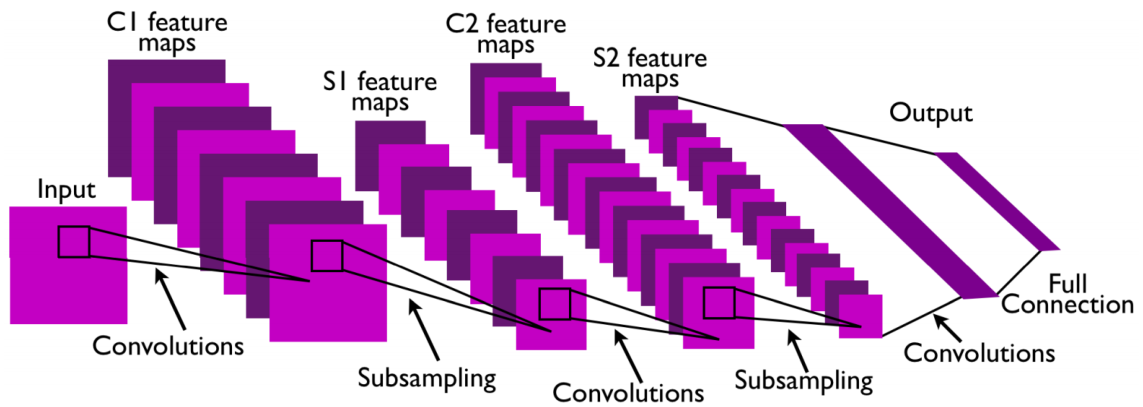
\includegraphics[width=15cm]{fig/ch2/conv1.png}
	\bicaption[\xiaosi 标准卷积网络结构示意图]{\wuhao 标准卷积网络结构示意图}{\wuhao Illustration of the structure of a standard convolutional network}
	\label{fig:conv1}
\end{figure}

卷积神经网络的核心是卷积层,它通过卷积操作提取输入图像的特征。卷积操作是一种线性、平移不变的操作,它通过在输入信号上进行局部加权组合来捕获不同的特征。卷积操作的参数是卷积核,不同的卷积核可以捕获图像的不同特征,例如边缘、纹理和形状等。卷积层的输出被送入激活函数进行非线性变换,以增加网络的表达能力。

除了卷积层,池化层也是卷积神经网络中的重要组成部分。池化层通过对卷积层的输出进行下采样,减少特征图的尺寸,同时保留最显著的特征。这有助于使网络对输入的位置变化具有一定的不变性,同时减少了参数数量,提高了计算效率。

全连接层通常位于网络的末尾,用于将卷积层和池化层提取的特征映射转换为最终的分类或回归结果。全连接层将所有特征进行组合,最终输出网络对输入的预测结果。


\section{基于Transformer的图像分类神经网络}
Transformer\textsuperscript{\cite{bengio2013representation}}是一种基于自注意力机制的深度学习模型架构,最初由A.Vaswani等人于2017年提出\textsuperscript{\cite{vaswani2017attenion}},被广泛应用于自然语言处理任务,如机器翻译、文本生成和语言建模等。相较于传统的循环神经网络(RNN)和卷积神经网络(CNN),Transformer在处理长距离依赖性和并行计算方面具有显著优势,成为了当今深度学习领域的研究热点。

Transformer模型的核心思想是完全基于注意力机制来实现信息的传递和组合。在传统的神经网络结构中,信息的传递是通过固定的层次顺序进行的,而Transformer则引入了自注意力机制,使得模型可以在不同位置之间建立动态的注意力联系。这种注意力机制使得模型能够更好地捕捉输入序列中不同位置之间的依赖关系,从而提高了模型在处理长距离依赖性任务时的性能。

如图\ref{fig:vit1}所示,Transformer模型由编码器和解码器两部分组成,每部分都包含多层的注意力机制模块。在编码器中,输入序列首先通过一个自注意力层,然后再通过一个全连接前馈神经网络层。在自注意力层中,每个输入位置都可以与其他位置建立注意力联系,从而使得模型能够同时考虑到整个输入序列的信息。在解码器中,除了编码器的结构外,还引入了一个额外的注意力层,用来对编码器的输出进行进一步处理。

除了自注意力机制,Transformer还引入了位置编码来表示输入序列中不同位置的信息。由于Transformer没有显式的循环结构,无法像RNN一样自然地捕捉序列中的位置信息,因此位置编码的引入可以帮助模型更好地理解输入序列中不同位置的相对位置关系。

另一个Transformer模型的重要特点是其并行计算能力。由于自注意力机制的特性,Transformer可以高效地进行并行计算,加速模型的训练和推理过程。这使得Transformer在处理大规模数据和长序列任务时具有明显的优势。


\begin{figure}[h]
	\centering 
	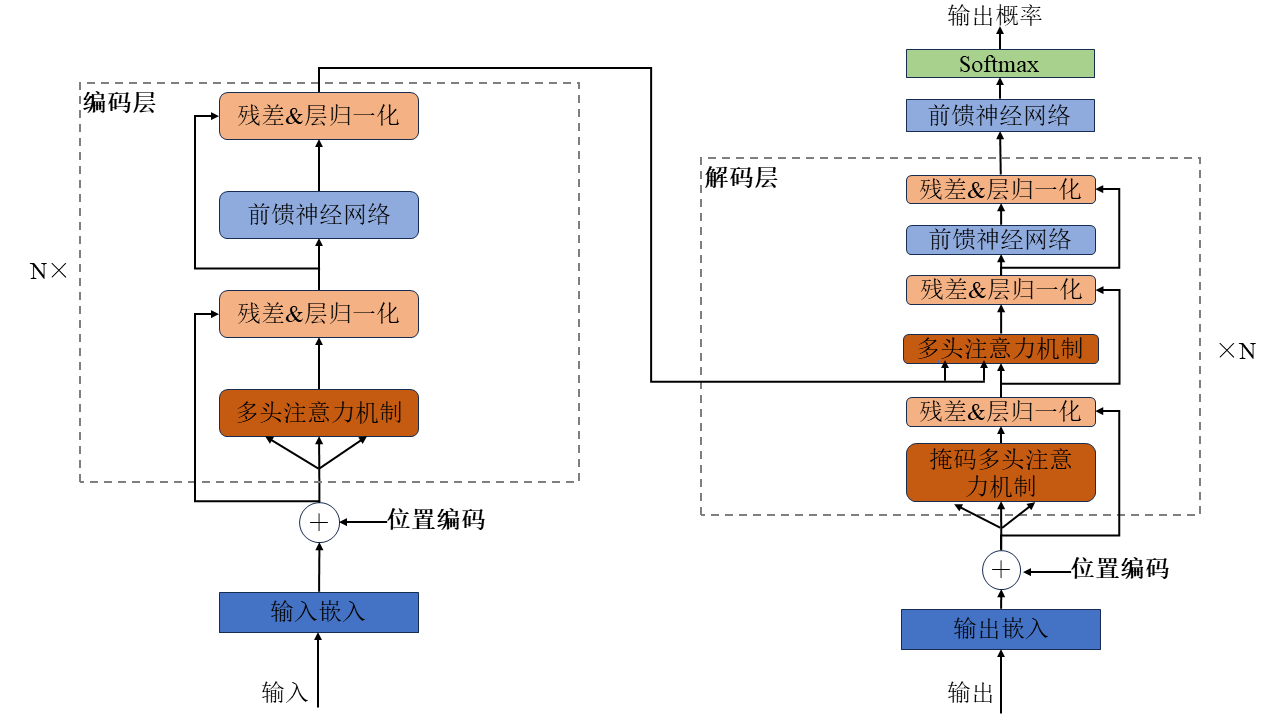
\includegraphics[width=15cm]{fig/ch2/vit1.png}
	\bicaption[\xiaosi Transformer结构示意图]{\wuhao Transformer结构示意图}{\wuhao Illustration of the structure of Transformer}
	\label{fig:vit1}
\end{figure}

\subsection{多头自注意力机制}
多头注意力机制是一种用于增强神经网络模型对输入序列的表示能力的技术。它通过将注意力机制应用于多个头部(head)来并行处理不同的注意力表示,从而提高模型的泛化能力和性能。多头注意力机制最早由Vaswani等人在Transformer模型中提出,并在自然语言处理领域取得了巨大成功。

多头注意力机制的基本原理是将输入序列分别映射到多个不同的查询、键和值空间,并通过计算每个头部的注意力权重来融合不同的信息。具体来说,多头注意力机制可以表示为以下公式:
\begin{equation}
	\text{MultiHead}(Q, K, V) = \text{Concat}(\text{head}_1, ..., \text{head}_h)W^O
\end{equation}



其中,$Q, K, V$分别表示输入序列的查询、键和值,$h$表示头部的数量,$\text{head}_i$表示第$i$个头部的注意力表示,$W^O$是输出权重矩阵。

在多头注意力机制中,每个头部都有自己的查询、键和值权重矩阵,通过线性变换将输入序列映射到不同的空间。然后,每个头部分别计算注意力权重,并将不同头部的注意力表示进行拼接,最后通过输出权重矩阵$W^O$融合多个头部的信息。

多头注意力机制的优势在于可以提高模型对不同部分的关注度,从而更好地捕捉输入序列中的重要信息。通过并行计算多个头部的注意力表示,模型可以更好地处理长距离依赖关系和复杂的序列结构,提高模型的泛化能力和性能。除了在Transformer模型中应用多头注意力机制,它还被广泛应用于其他神经网络模型中,如BERT\textsuperscript{\cite{kenton2019bert}}、GPT\textsuperscript{\cite{floridi2020gpt}}等。在自然语言处理、计算机视觉等领域,多头注意力机制已成为提高模型性能的重要技术之一。
 
\subsection{编码器}
Transformer模型是一种基于注意力机制的神经网络模型,由编码器和解码器组成,广泛应用于自然语言处理领域。编码器是Transformer模型的核心组件之一,它负责将输入序列转换成隐藏表示,提供给解码器进行生成输出序列。编码器由多个编码器层堆叠而成,每个编码器层内部包含多头自注意力机制和前馈神经网络。

编码器的每一层都包含两个子层,分别是多头自注意力机制和前馈神经网络。下面分别介绍编码器每一层的计算过程:

1. 多头自注意力机制(Multi-Head Self-Attention):

多头自注意力机制是编码器每一层的第一个子层,用于计算输入序列的注意力表示。具体的计算过程可以表示为以下公式:

\begin{equation}
	\text{Attention}(Q, K, V) = \text{softmax}\left(\frac{QK^T}{\sqrt{d_k}}\right)V
\end{equation}

其中,$Q, K, V$分别表示输入序列的查询、键和值,$d_k$表示注意力头部的维度。在多头自注意力机制中,将输入序列分别映射到多个不同的查询、键和值空间,并通过计算每个头部的注意力权重来融合不同的信息。

2. 前馈神经网络(Feed-Forward Neural Network):

前馈神经网络是编码器每一层的第二个子层,用于对注意力表示进行非线性变换。具体的计算过程可以表示为以下公式:

\begin{equation}
	\text{FFN}(x) = \text{ReLU}(xW_1 + b_1)W_2 + b_2
\end{equation}


其中,$x$表示输入的注意力表示,$W_1, b_1, W_2, b_2$分别表示两个线性变换的权重和偏置。前馈神经网络通过两个线性变换和ReLU激活函数来对注意力表示进行非线性变换,从而提高模型的表征能力。

在编码器中,每个编码器层都包含多头自注意力机制和前馈神经网络这两个子层,通过堆叠多个编码器层来构建整个编码器。每个编码器层都可以表示为以下公式:
\begin{equation}
	\text{EncoderLayer}(x) = \text{FFN}(\text{Attention}(x) + x)
\end{equation}

其中,$x$表示输入序列的隐藏表示,$\text{Attention}(x)$表示多头自注意力机制的输出,$\text{FFN}(\cdot)$表示前馈神经网络的输出。通过将多头自注意力机制的输出和原始输入序列相加,并通过前馈神经网络进行非线性变换,编码器可以逐层提取输入序列的特征表示。

在Transformer模型的编码器中,除了多头自注意力机制和前馈神经网络之外,还包括残差连接和层归一化这两个重要的组件。残差连接和层归一化在每个编码器层中都起着重要的作用,有助于提高模型的训练稳定性和加速收敛。下面分别介绍这两个组件的作用和公式表达:


3. 残差连接(Residual Connection):

残差连接是指将输入序列的隐藏表示与经过子层处理后的表示进行相加,从而形成残差连接。这样的设计有助于减轻梯度消失和梯度爆炸的问题,提高模型的训练效果。残差连接的计算公式可以表示为:

\begin{equation}
	\text{Residual}(x, \text{Sublayer}(x)) = x + \text{Sublayer}(x)
\end{equation}


其中,$x$表示输入序列的隐藏表示,$\text{Sublayer}(x)$表示经过子层处理后的表示。通过残差连接,编码器每一层的输出可以保留原始输入序列的信息,同时加入子层处理后的新信息,从而提高模型的表征能力。

4. 层归一化(Layer Normalization):

层归一化是一种对神经网络中每一层输出进行归一化的技术,有助于加速模型的收敛和提高模型的泛化能力。在编码器的每个子层(包括多头自注意力机制和前馈神经网络)后都会应用层归一化操作。层归一化的计算公式可以表示为:
\begin{equation}
	\text{LayerNorm}(x) = \gamma \odot \frac{x - \mu}{\sqrt{\sigma^2 + \epsilon}} + \beta
\end{equation}


其中,$x$表示输入序列的隐藏表示,$\gamma$和$\beta$分别表示学习到的缩放因子和偏置项,$\mu$和$\sigma$分别表示输入的均值和标准差,$\epsilon$是一个很小的常数,避免分母为零。层归一化通过对每一层的输出进行归一化,有助于减少内部协变量转移,提高模型的训练效果。

\subsection{解码器}
在Transformer模型中,解码器是用于生成目标序列的部分,与编码器相对应。解码器由多个解码器层组成,每个解码器层包含掩码多头自注意力机制、多头自注意力机制、层归一化、残差连接、前馈神经网络。此处重点介绍一下掩码多头自注意力机制(Masked Multi-Head Self-Attention)。

在Transformer模型中,掩码多头自注意力机制是解码器中的关键组件之一,它允许解码器在生成目标序列时关注目标序列中的不同位置,并避免未来信息的干扰。掩码多头自注意力机制包含多个注意力头,每个头都学习不同的注意力权重,然后将它们合并起来以获得最终的注意力表示。

在掩码多头自注意力机制中,给定一个输入序列$X = \{x_1, x_2, ..., x_n\}$,我们首先通过线性变换得到查询(Query)、键(Key)和值(Value)的表示:
\begin{equation}
Q = XW^Q, \ K = XW^K, \ V = XW^V
\end{equation}
其中$W^Q, W^K, W^V$是学习的权重矩阵。接下来,计算每个注意力头的注意力分数$A_i$:
\begin{equation}
A_i = \text{softmax}(\frac{Q_iK_i^T}{\sqrt{d_k}})
\end{equation}
其中$Q_i, K_i$表示第$i$个注意力头的查询和键,$d_k$是键的维度。然后,将每个注意力头的注意力分数与值相乘并加权求和,得到最终的输出表示:
\begin{equation}
\text{MultiHead}(Q, K, V) = \text{Concat}(\text{head}_1, ..., \text{head}_h)W^O
\end{equation}
其中$\text{head}_i = \text{Attention}(QW_i^Q, KW_i^K, VW_i^V)$表示第$i$个注意力头的输出,$W^O$是最终的输出权重矩阵。

在掩码多头自注意力机制中,为了避免未来信息的泄露,会对注意力分数进行掩码操作。具体来说,在计算注意力分数时,会将当前位置之后的信息屏蔽掉,以确保模型只能使用当前位置之前的信息。在实际操作中是将输入矩阵加上一个上三角矩阵,该上三角矩阵元素为无穷大。这种掩码操作有助于解码器在生成目标序列时保持因果关系,不受未来信息的影响。

通过掩码多头自注意力机制,解码器可以有效地关注目标序列中的不同部分,并根据输入序列和先前生成的部分序列调整生成的单词,从而实现对目标序列的准确生成。
\subsection{应用于图像分类领域的Transformer}
Transformer 技术最初是为了处理自然语言处理任务而设计的,但随着其出色的性能和可扩展性,人们开始将 Transformer 技术应用于其他领域,包括图像分类。虽然传统的卷积神经网络(CNN)在图像分类任务中表现出色,但 Transformer 在图像分类领域也展示出了很好的潜力。

在图像分类领域应用 Transformer 技术的一个主要方法是 Vision Transformer(ViT)\textsuperscript{\cite{dosovitskiy2020image}}。ViT 将输入的图像像素视为序列化的数据,然后利用 Transformer 模型来对序列化的图像数据进行处理。ViT 的基本架构如下:

图像块划分:将输入图像分成固定大小的图像块(patches),每个图像块将被视为一个 token。
输入嵌入层:将每个图像块映射为一个向量表示。
位置编码:为每个图像块的向量表示添加位置编码,以保留图像块之间的位置信息。
Transformer 编码器:使用 Transformer 模型对序列化的图像数据进行处理,包括多层的自注意力机制和前馈神经网络。
分类头:将 Transformer 的输出通过一个全连接层进行分类,得到图像的类别预测。

ViT 在图像分类领域的应用有以下优点:可扩展性:Transformer 模型的自注意力机制使得 ViT 能够捕捉图像中的全局信息,而不受卷积核大小的限制。灵活性:ViT 可以处理不同尺寸的图像,而无需调整网络结构。泛化能力:ViT 在处理小样本数据集时表现较好,因为 Transformer 模型具有强大的表示学习能力。ViT的结构如图\ref{fig:vit2}所示。

\begin{figure}[h]
	\centering 
	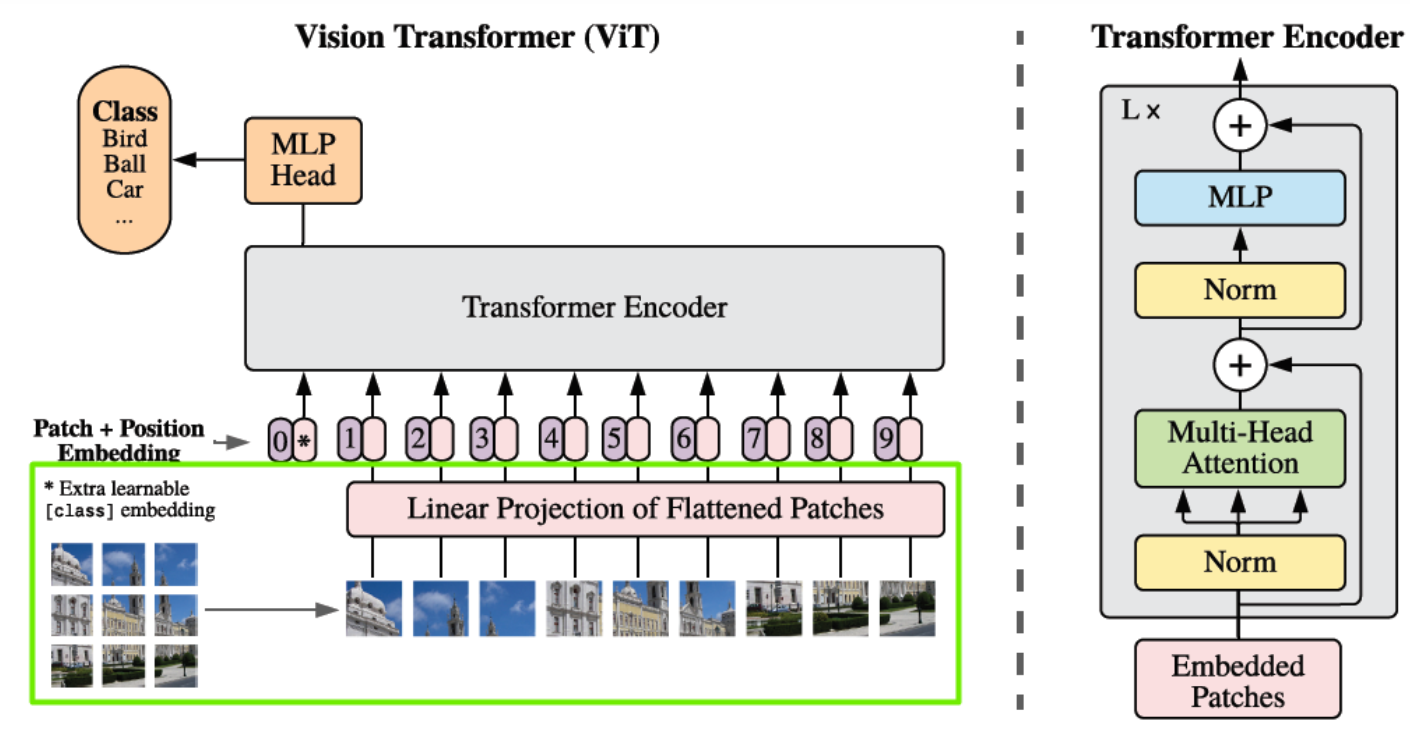
\includegraphics[width=15cm]{fig/ch2/vit2.png}
	\bicaption[\xiaosi ViT结构示意图]{\wuhao ViT结构示意图}{\wuhao Illustration of the structure of ViT}
	\label{fig:vit2}
\end{figure}


\section{常见的显著图解释方法}
本节将会介绍五种著名的显著图解释方法,包括Grad-CAM\textsuperscript{\cite{selvaraju2017grad}}、Grad-CAM++\textsuperscript{\cite{chattopadhay2018grad}}、Score-CAM\textsuperscript{\cite{wang2020score}}、LRP\textsuperscript{\cite{binder2016layer}}和Transformer attribution\textsuperscript{\cite{chefer2021transformer}}。本节将会介绍这五种方法的具体理论依据,各自的应用条件和算法流程。 
\subsection{Grad-CAM}\label{sub:gradcam}
Grad-CAM(Gradient-weighted Class Activation Mapping)是一种用于解释深度学习模型的方法,它能够生成图像级别的重要区域热力图,从而帮助理解模型的决策过程。Grad-CAM的主要优点是它不需要对模型进行修改,可以应用于任何卷积神经网络模型,并且能够提供直观的可视化结果。

Grad-CAM的核心思想是利用模型的梯度信息和特征图信息来推导出图像中哪些区域对于模型的分类决策最为关键。在深度学习模型中,每个卷积层都可以看作是对输入图像进行特征提取的过程,因此可以通过分析梯度信息来了解哪些特征对于模型的分类决策起到了关键作用。之前的一些研究已经断言,卷积神经网络的更深层表征捕获了更高层次的视觉结构\textsuperscript{\cite{bengio2013representation,mahendran2016visualizing}}。此外,卷积层自然地保留了在全连接层中丢失的空间信息,因此Grad-CAM的作者认为最后一层卷积层在高级语义和详细空间信息之间有良好的表现。因此Grad-CAM使用流入卷积神经网络最后一个卷积层的梯度信息,为每个神经元分配一个特定感兴趣的决策的重要性值。虽然Grad-CAM的技术相当通用,因为它可以用来解释深度网络任何层的激活,但是一般来说它用来可视化解释输出层做的决定。

\begin{figure}[h]
	\centering 
	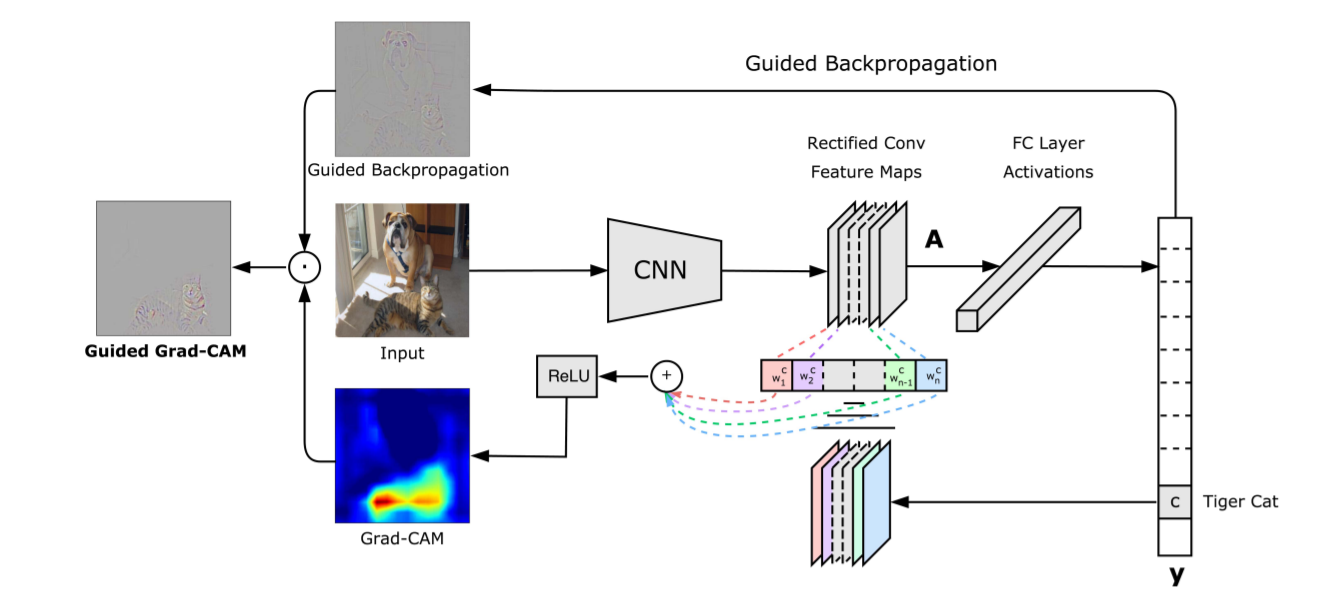
\includegraphics[width=15cm]{fig/ch2/gradcam1.png}
	\bicaption[\xiaosi Grad-CAM流程示意图]{\wuhao Grad-CAM流程示意图}{\wuhao Pipeline of  Grad-CAM}
	\label{fig:gradcam1}
\end{figure}

下面详细解释一下Grad-CAM的计算过程。若假设$I \in \mathbb{R}^{3\times H \times W}$是输入图片, $\mathcal{F}$是预训练好的基于卷积神经网络的图像分类模型,$\mathcal{F}_c(I)$ 表示输入图片是$I$的情况下模型$\mathcal{F}$输出的关于类别索引$c$的分数(该分数未经softmax函数)。对于给定的模型$\mathcal{F}$卷积层$l$,在图片$I$输入到模型$\mathcal{F}$前向传播过程中可以从卷积层$l$提取特征图集合$\overset{*}{\bm{A}}$。为了获取具有类别区分性的显著图,Grad-CAM首先需要计算关于类别$c$的梯度,为了得到 $\mathcal{F}_c(I)$ 相对于 第$k$张特征图 $A^k \in \overset{*}{\bm{A}}$ 的梯度,我们可以对 $\mathcal{F}_c(I)$ 进行反向传播。为了得到每个特征图的重要性权重,梯度会在高度和宽度两个维度上进行全局平均。
\begin{equation}
	w^c_k=\frac{1}{m\times n}\sum_{i=1}^{m}\sum_{j=1}^{n}\frac{\partial \mathcal{F}_c(I)}{\partial A_{ij}^k(I)}
	\label{eq:gradcam_wk}
\end{equation}
式子\ref{eq:gradcam_wk}表示了特征图集合中特征图$A^k$的权重计算方式,其中,$A_{ij}^k$ 表示 第$k$张特征图中 第$i$ 行和 第$j$ 列的值,$m$ 和 $n$ 分别是梯度矩阵的宽度和高度。$w^c_k \in \overset{*}{\bm{W}}$ 是 第$k$张 特征图的权重。$\overset{*}{\bm{W}}$是大小为$K$的一维向量,$K$是$\overset{*}{\bm{A}}$的通道数。


$w^c_k $的含义表示第$k$张特征图在后续计算中对输出分数$\mathcal{F}_c(I)$的贡献程度。最后将每张特征图和其权重相乘然后将相乘结果进行线性组合,最后通过ReLU函数即可得到Grad-CAM的显著图。具体计算方式如下所示:
\begin{equation}
	L_{Grad-CAM}=ReLU(\sum_K(w^c_k A^k))
	\label{eq:gradcam}
\end{equation}
需要注意的是注意,这会产生一个与特征图$A^k$尺寸大小相同的原始显著图,若需要将其展示重叠在输入图片上,应该将其进行上采样。还有就是ReLU函数应用于显著图的线性组合,是因为Grad-CAM只对感兴趣的类别有积极影响的特征感兴趣,即类别索引$c$所代表的类别。原始显著图中为负值的像素可能属于图像中的其他类别。若没有这个ReLU函数,显著图中会将其他不相干的类别进行凸显。图\ref{fig:gradcam1}简要展示了Grad-CAM的工作流程。


\subsection{Grad-CAM++}
在原始的CAM\textsuperscript{\cite{zhou2016learning}}方法中每张特征图的权重$w^c_k$是通过最后一层卷积层生成的特征图来训练线性分类器来获得的,但是其局限是必须使用全局平均池化层,需要重新训练模型,Grad-CAM解决了这一问题,通过最后的类别分数反向传播对最后一层卷积层的特征图求导,利用单个梯度矩阵的平均值来得到单张特征图权重,但是这会导致其对于某张特征图加权值过大从而将其他包含目标物体特征的特征图权值过小,从而在最后生成的显著图上忽略关键的特征。图\ref{fig:gradcampp1}举例说明了这一现象,如图所示,图中黑色方块部分表示目标物体在图中二维空间上特征分布,最后经过卷积层生成3个特征图分布是$A^1$、$A^2$和$A^3$,其中$A^1$特征图的特征区域占比最多,$A^2$和$A^3$的特征区域明显较少,如果使用Grad-CAM的加权方式则最后的生成的显著图会将$A^2$和$A^3$的特征区域弱化甚至忽略,这显然是不对的。这种情况一般会出现在有多个目标物体的图片当中。
\begin{figure}[h]
	\centering 
	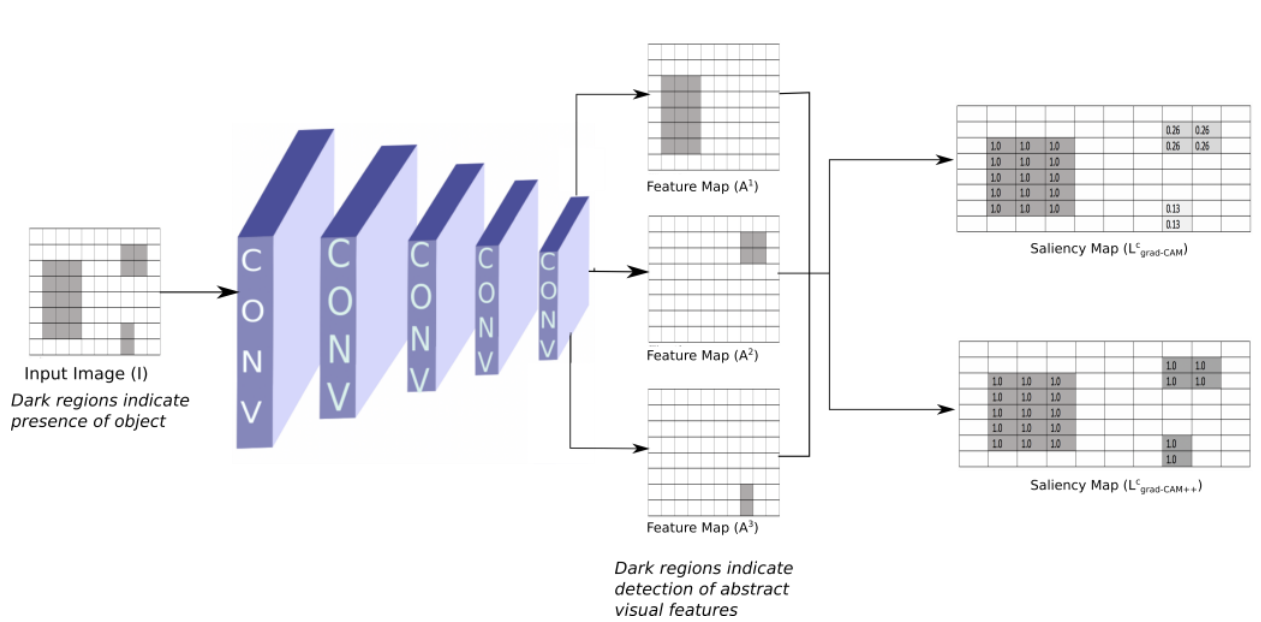
\includegraphics[width=15cm ]{fig/ch2/gradcampp1.png}
	\bicaption[\xiaosi 一个假设性的例子说明Grad-CAM++的优势]{\wuhao 一个假设性的例子说明Grad-CAM++的优势}{\wuhao A hypothetical example elucidating the intuition behind Grad-CAM++}
	\label{fig:gradcampp1}
\end{figure}


Grad-CAM++为了解决这一现象则没有直接将梯度矩阵直接全剧平均池化取平均值来作为特征图权重,而且为梯度矩阵上每一个元素赋予了一个权重,之后将梯度矩阵上的元素值全部相加取和作为特征图权重。具体的权重表示公式如下:
\begin{equation}
	w_{k}^{c}=\sum_{i} \sum_{j} \alpha_{i j}^{k c} \cdot \operatorname{ReLU}\left(\frac{\partial Y^{c}}{\partial A_{i j}^{k}}\right)  
	\label{eq:gradcampp_wkc}
\end{equation}
式\ref{eq:gradcampp_wkc}中$Y^{c}$即和章节\ref{sub:gradcam}$中\mathcal{F}_c(I)$含义一致,均表示输入图片进入模型中,模型输出的关于类别索引$c$的分数。$i$和$j$表示特征图中的$A^{k}$的行列迭代器。式\ref{eq:gradcampp_wkc}中$\alpha_{i j}^{k c}$的具体计算方式如下:
\begin{equation}
	\alpha_{i j}^{k c}=\frac{\frac{\partial^{2} Y^{c}}{\left(\partial A_{ij}^{k}\right)^{2}}}{2 \frac{\partial^{2} Y^{c}}{\left(\partial A_{i j}^{k}\right)^{2}}+\sum_{a} \sum_{b} A_{a b}^{k}\frac{\partial^{3} Y^{c}}{\left(\partial A_{i j}^{k}\right)^{3}}}
	\label{eq:gradcampp_akc}
\end{equation}
\begin{figure}[h]
	\centering 
	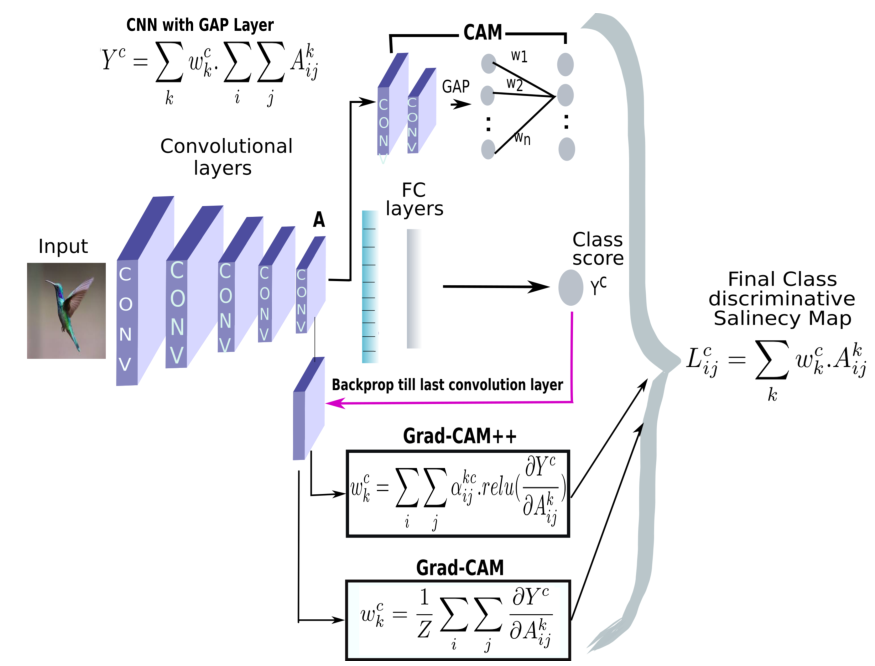
\includegraphics[width=15cm]{fig/ch2/gradcampp2.png}
	\bicaption[\xiaosi CAM, Grad-CAM, Grad-CAM++的各自计算方式]{\wuhao CAM, Grad-CAM, Grad-CAM++的各自计算方式}{\wuhao Respective calculations for CAM, Grad-CAM, Grad-CAM++}
	\label{fig:gradcampp2}
\end{figure}
将式\ref{eq:gradcampp_akc}和式\ref{eq:gradcampp_wkc}结合即可得到如下完整的权重计算公式:
\begin{equation}
	w_{k}^{c}=\sum_{i} \sum_{j}\left[\frac{\frac{\partial^{2} Y^{c}}{\left(\partial A_{i j}^{k}\right)^{2}}}{2 \frac{\partial^{2} Y^{c}}{\left(\partial A_{i j}^{k}\right)^{2}}+\sum_{a} \sum_{b} A_{a b}^{k}\frac{\partial^{3} Y^{c}}{\left(\partial A_{i j}^{k}\right)^{3}}}\right] \cdot \operatorname{ReLU}\left(\frac{\partial Y^{c}}{\partial A_{i j}^{k}}\right)
\end{equation}
得到权重后,将权重$w_{k}^{c}$和其对应的特征图$A^k$相乘,然后所有特征图线性相加即可得到Grad-CAM++生成的最终显著图。计算过程和式\ref{eq:gradcam}一致。图\ref{fig:gradcampp2}中展示了CAM、Grad-CAM、Grad-CAM++的权重计算方式异同。


\subsection{Score-CAM}
Grad-CAM和Grad-CAM++都依赖反向传播的梯度作为权重,但是这种基于梯度的方法也有缺点,若激活函数是Sigmoid函数或者ReLU函数,则会分别带来梯度饱和以及梯度消失的问题\textsuperscript{\cite{simonyan2014visualising}},反映到显著图上就是会导致噪声问题。此外依靠梯度作为权重也存在不可靠的问题,如图\ref{fig:scorecam1}所示,在这幅图中(2)(3)(4)分别是对应的特征图上采样后叠加到原图上,其中没有遮盖的部分表示该特征图在原图上较为关注的特征区域,将(2)(3)(4)通过图像分类模型,得到对应类别的得分分别是 0.003,0.999,0.997。从结果上看,(3)(4)的特征图关注的区域对于该类别是比较重要的。然而在生成Grad-CAM的显著图时,这三者计算出的权重分别是0.035,0.027,0.021。反而是对于结果影响很小的(2)的特征图权重更高。这就显示出了基于梯度的类激活映射方法的不足。


\begin{figure}[h]
	\centering 
	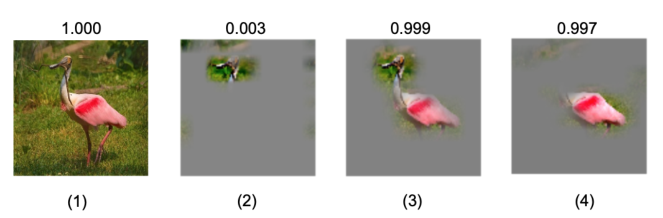
\includegraphics[width=15cm]{fig/ch2/scorecam1.png}
	\bicaption[\xiaosi 特征图扰动示例]{\wuhao 特征图扰动示例}{\wuhao Example of feature map perturbation}
	\label{fig:scorecam1}
\end{figure}

因此Score-CAM不依赖于梯度来获得特征图线性加权的权重,而是通过每张特征图在目标类上的前向传播的概率分数来获得每张特征图的权重。下面通过具体的定义来说明Score-CAM的计算方式。当输入图片为$I \in \mathbb{R}^{3\times H \times W}$时,图像分类模型为$\mathcal{F}$时,经过前向传播从指定卷积层$l$提取的第$k$个通道的特征图为$A^k_l$,那么该特征图对于指定类别$c$的概率分数$\mathcal{F}_c(I)$的贡献程度,即$A^k_l$权重$C(A^k_l)$可以由以下式子计算得出:
\begin{equation}
	C(A^k_l)=\mathcal{F}_c(I \circ H(^k_l))-\mathcal{F}_c(I_b)
	\label{eq:scorecam_C}
\end{equation}
式子\ref{eq:scorecam_C}中,$I_b$表示一张基准图像,该图像要求在类别索引$c$上的概率值尽可能的小,即$\mathcal{F}_c(I_b)$的值趋近于0,在算法实际实施的过程当中,该基准图片$I_b$一般是值均为0的全黑图像。$\circ$表示哈达玛积运算,即运算符两边的矩阵对应位置元素相乘,$H(^k_l)$是$A^k_l$上采样后的图片。其计算式子如下所示:
\begin{equation}
	H(^k_l)=s(U\!p(A^k_l))
	\label{eq:scorecam_H}
\end{equation}
式\ref{eq:scorecam_H}中,$U\!p$表示上采样运算,此处是将特征图其$A^k_l$上采样至原始输入图片尺寸。$s$表示对图片进行归一化运算,将图片中的所有像素值控制在$[0,1]$。最后可以得到Score-CAM的显著图计算式子:
\begin{equation}
	L_{\text {Score-CAM }}^{c}=\operatorname{ReLU}\left(\sum_{k} \alpha_{k}^{c} A_{l}^{k}\right)
	\label{eq:scorecam_L}
\end{equation}
式\ref{eq:scorecam_L}中,权值$\alpha_{k}^{c}$即表示$C(A^k_l)$。Score-CAM和Grad-CAM,Grad-CAM++最大的不同就是它创新性的利用特征图作为扰动输入图片的掩膜,以网络模型关于指定类别的概率分数来作为每张特征图的权重。


\subsection{LRP}
LRP全称为Layer-wise relevance propagation,意思是层间相关性传播,是深度学习中用于理解和解释神经网络决策的一种技术。LRP的主要思想是通过赋予输出结果一个相关性的分数,然后定义反向传播规则,将该相关分数逐层向后传播,通过计算给每层的每个神经元赋予一个相关性分数来表示它对输出结果的贡献程度,传播回输入层即可得到输入图片中每个像素的相关性分数,分数值的大小表示该像素与最终决策结果的相关性程度,也即贡献程度。利用获得的输入图片的每个像素的相关性分数也可以生成显著图。在传播过程中每层网络的神经元的相关性分数总和是一致的。通过这样做,LRP有助于揭示每个输入特征对最终决策的贡献,为神经网络的内部运作提供宝贵的见解。LPR的主要思想遵循以下公式:
\begin{equation}
	f(x)\approx \sum_{d=1}^{V} R_d
	\label{eq:lrp_fx}
\end{equation}
式\ref{eq:lrp_fx}中$f(x)$ 表示输入图片是$x$的情况下,其中某一个特定类别在图片$x$中的存在概率。$R_d$ 表示图片中单一像素点对该类别的相关性分数,可以看作是贡献值。图\ref{fig:lrp1}大体展示了这种分解思想。图像$x$被转换为一串特征向量,并应用分类器将图像归入给定类别,如“猫”或 “无猫”,该图中将“猫”的分类结果概率分数作为总的相关性分数反向传播至输入图片中的每个像素,最终可以得到可视化单个像素对预测的贡献。
\begin{figure}[h]
	\centering 
	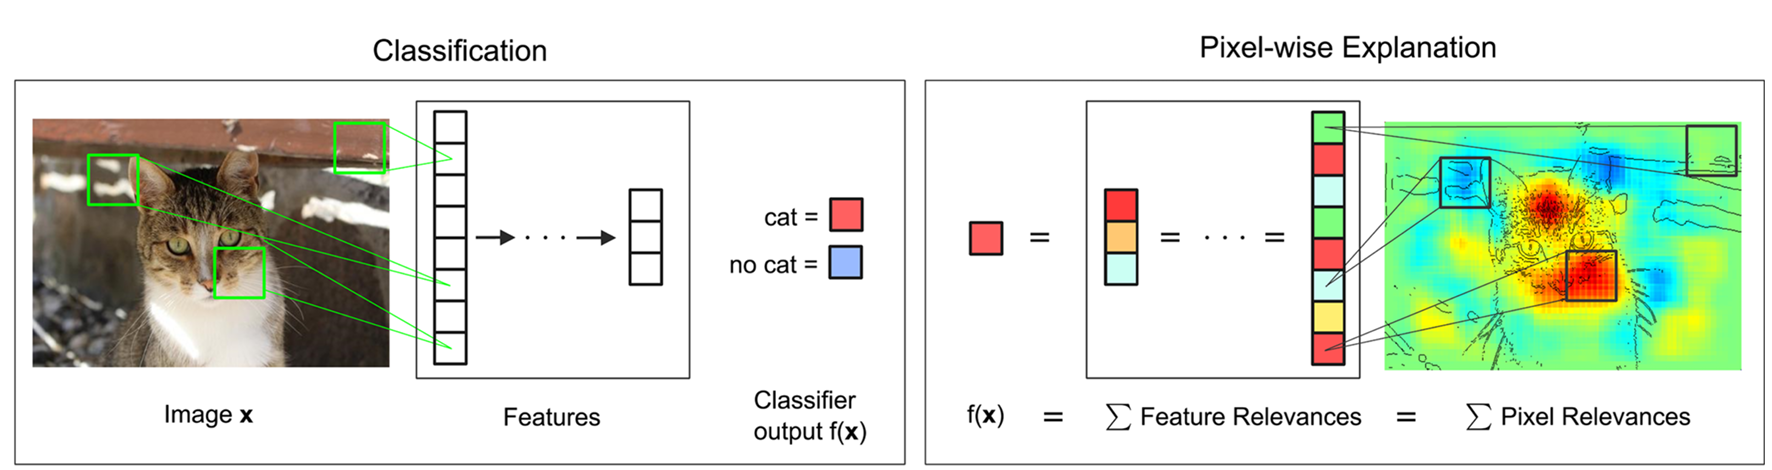
\includegraphics[width=15cm]{fig/ch2/lrp1.png}
	\bicaption[\xiaosi 像素相关性分解过程可视化]{\wuhao 像素相关性分解过程可视化}{\wuhao Visualization of the pixel relevance decomposition process}
	\label{fig:lrp1}
\end{figure}

下面结合公式推导详细说明LRP的计算过程。对于图像分类神经网络关于某个类别的输出$f(x)$有以下规则,每层的所有神经元的相关性分数是相等的。
\begin{equation}
	f(x)=\ldots=\sum_{d \in l+1} R_{d}^{l+1}=\sum_{d \in l} R_{d}^{l}=\ldots=\sum_{d} R_{d}^{1}
	\label{eq:lrp_fx2}
\end{equation}
式\ref{eq:lrp_fx2}中$l$表示神经网络的某一层,$l$越大越靠近输出层。

对于普通的多层神经网络,有如图\ref{fig:lrp2}所示的计算过程。其中:
\begin{equation}
	z_{ij}=x_iw_{ij}
	\label{eq:lrp_zij}
\end{equation}
\begin{equation}
	z_{j}=\sum_i z_{ij}+b_j
	\label{eq:lrp_zj}
\end{equation}
\begin{equation}
	x_j=g(z_{j})
	\label{eq:lrp_xj}
\end{equation}

对于式\ref{eq:lrp_zij},神经元$i$乘以其和神经元$j$之间的权重$w_{ij}$得到中间计算结果$z_{ij}$。而式\ref{eq:lrp_zj}的值是第$i$层所有神经元和权重$w _{ij}$相乘后得到的$z_{ij}$的和加上偏置项$b_j$得到的。最后$z_j$经过激活函数$g$得到第$j$层某个神经元的值$x_j$。这三个式子的意思可以总结成所有上层神经元到下层的某个神经元$j$的值,也可以理解成贡献,决定了下层神经元$j$的中间值$z_j$,只不过最后要加上偏置项和经过激活函数。

\begin{figure}[h]
	\centering 
	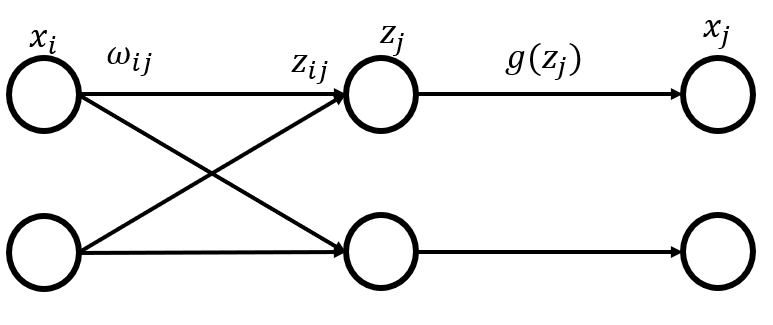
\includegraphics[width=15cm]{fig/ch2/lrp2.png}
	\bicaption[\xiaosi 多层神经网络前向传播计算示例]{\wuhao 多层神经网络前向传播计算示例}{\wuhao Example of a multilayer neural network forward propagation calculation}
	\label{fig:lrp2}
\end{figure}



从以上前向传播的示例过程中可以推导出LRP相关性传播的基本过程,如图\ref{fig:lrp3}所示,左半部分是前向传播的过程,右半部分是LRP的相关性反向传播的过程,其中$R_i^{(l)}$表示第$l$层神经元$i$的相关性分数,$R_{i\leftrightarrow j}^{(l,l+1)}$表示$l+1$层的某个神经元$j$的相关性等于$l+1$层的神经元$j$给$l$层所有神经元的相关性之和。下面结合图\ref{fig:lrp4}进行详细说明。
\begin{figure}[h]
	\centering 
	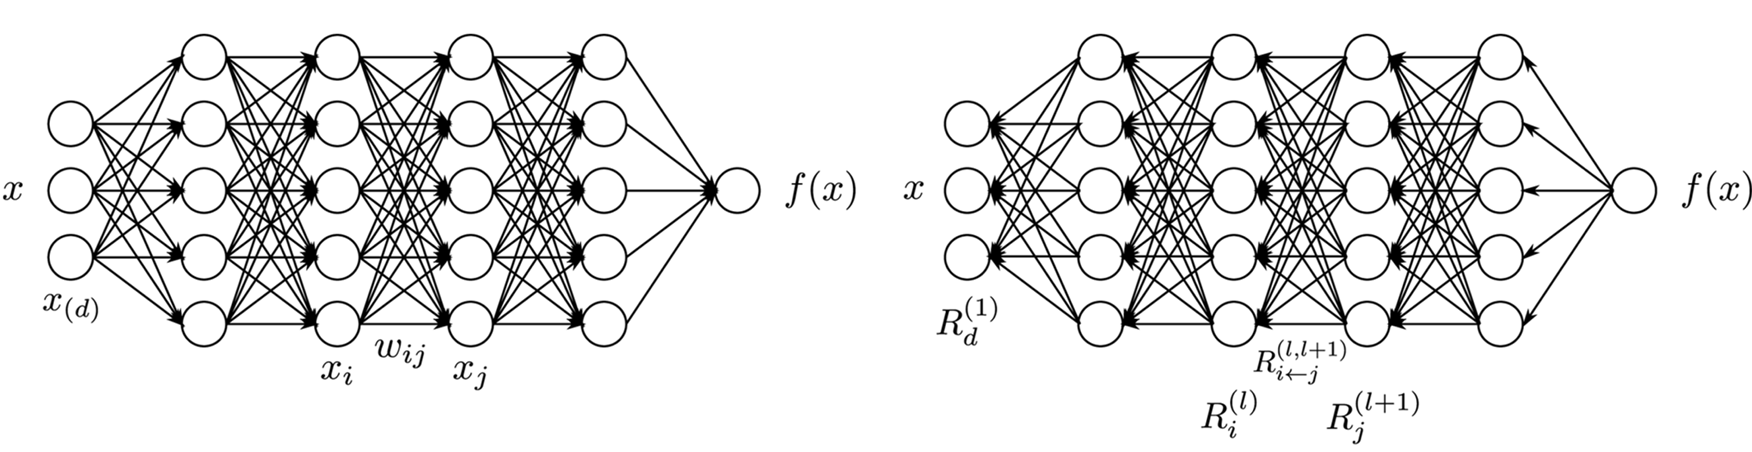
\includegraphics[width=15cm]{fig/ch2/lrp3.png}
	\bicaption[\xiaosi 多层神经网络下前向传播和层间相关性传播过程]{\wuhao 多层神经网络下前向传播和层间相关性传播过程}{\wuhao Forward propagation and LRP processes under multilayer neural networks}
	\label{fig:lrp3}
\end{figure}

\begin{figure}[h]
	\centering 
	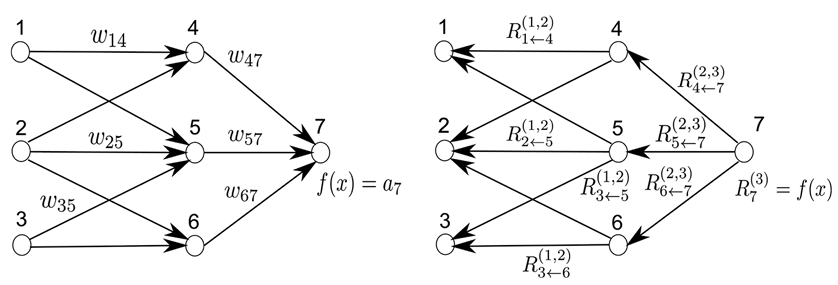
\includegraphics[width=15cm]{fig/ch2/lrp4.png}
	\bicaption[\xiaosi 层间相关性传播分配相关性分数的例子]{\wuhao 层间相关性传播分配相关性分数的例子}{\wuhao Example of LRP assigning relevance scores}
	\label{fig:lrp4}
\end{figure}
在图\ref{fig:lrp4}中的右半部分,第3层的7号神经元的相关性分数$R_{7}^{(3)}$相关性反向传播时是按照如下式子分配的:
\begin{equation}
	R_{7}^{(3)}=R_{4 \leftarrow 7}^{(2,3)}+R_{5 \leftarrow 7}^{(2,3)}+R_{6 \leftarrow 7}^{(2,3)}
\end{equation}
其中$R_{4 \leftarrow 7}^{(2,3)}$、$R_{5 \leftarrow 7}^{(2,3)}$和$R_{6 \leftarrow 7}^{(2,3)}$的值,也就是7号神经元分配给第二层的4,5和6号神经元的相关性分数在神经网络是线性的情况下(没有激活函数)可以结合公式\ref{eq:lrp_zij}进行计算,具体计算公式如下:
\begin{equation}
	R_{i \leftarrow j}^{(l, l+1)}=\frac{z_{i j}}{\sum_{i} z_{i j}} R_{j}^{(l+1)}
	\label{eq:lrp_Rij}
\end{equation}
式\ref{eq:lrp_Rij}的含义就是就是下层的神经元$j$的分配给上层神经元$j$相关性分数是$j$的总相关性分数乘以神经元$i$输出给$j$的值占$j$收到上层所有值的比。

但是在实际应用当中,神经网络会存在激活函数和偏置,式\ref{eq:lrp_Rij}无法完美应用。考虑到激活函数是双曲正切$Tanh(x)$和$ReLU$函数的情况,可以用以下公式取近似值:
\begin{equation}
	R_{i \leftarrow j}^{(l, l+1)}=\frac{z_{i j}}{z_{j}} R_{j}^{(l+1)}
\end{equation}
其他激活函数情况可以使用如下式子计算:
\begin{equation}
	\sum_{i} R_{i \leftarrow j}^{(l, l+1)}=R_{j}^{(l+1)} \cdot\left(1-\frac{b_{j}}{z_{j}}\right)
\end{equation}

\subsection{Transformer attribution}
Transformer attribution是H.Chefer等人\textsuperscript{\cite{chefer2021transformer}}于近些年提出的针对基于Transformer架构的深度神经网络的可解释方法,其在图像分类神经网络上也能够生成质量较高的显著图。Transformer attribution针对Transformer的特殊结构改进了传统的LRP算法,针对相关性反向传播过程中的注意力层和残差连接的提出了特殊的LRP传播规则,同时将其应用到基于Transformer的图片分类模型中,相比之前的可视化算法,Transformer attribution得到了较为可靠的显著图结果。

下面是Transformer attribution的详细推导过程。对于LRP传播,总是遵守以下规则:
\begin{equation}
	\sum_{j} R_{j}^{(n)}=\sum_{i} R_{i}^{(n-1)}
\end{equation}
即每层的相关性分数总和总是相等的。


若用$L^{(n)}(\mathbf{X},\mathbf{Y})$表示层对两个张量$\mathbf{X}$和$\mathbf{Y}$的操作。通常,这两个张量是第$n$层的输入特征映射和权重。则LRP遵循通用深度泰勒分解\textsuperscript{\cite{montavon2017explaining}}的规则,具体如下表示:

\begin{equation}
	R_{j}^{(n)} =\mathcal{G}\left(\mathbf{X}, \mathbf{Y}, R^{(n-1)}\right) =\sum_{i} \mathbf{X}_{j} \frac{\partial L_{i}^{(n)}(\mathbf{X}, \mathbf{Y})}{\partial \mathbf{X}_{j}} \frac{R_{i}^{(n-1)}}{L_{i}^{(n)}(\mathbf{X}, \mathbf{Y})}
	\label{eq:trans_Rnj1}
\end{equation}
对于激活函数是ReLU的情况,第$n$层的第$j$个神经元的相关性分数可以如下计算:
\begin{equation}
	R_{j}^{(n)}=\mathcal{G}\left(x^{+}, w^{+}, R^{(n-1)}\right)=\sum_{i} \frac{x_{j}^{+} w_{j i}^{+}}{\sum_{j^{\prime}} x_{j^{\prime}}^{+} w_{j^{\prime} i}^{+}} R_{i}^{(n-1)}
	\label{eq:trans_Rnj2}
\end{equation}
式\ref{eq:trans_Rnj1}和式\ref{eq:trans_Rnj2}中,$j$是和第$n$层的神经元对应的,$i$和第$n-1$层的神经元对应,$j^{\prime}$是第$n$层神经元的取和过程中的迭代计数符号。加号表示只保留正值,计算方式为$max(0,x)$。但是Transformer使用的是GELU函数,有正值也有负值同时也是非线性函数。其相关性分数计算方式如下:
\begin{equation}
	R_{j}^{(n)}  =\mathcal{G}_{q}\left(x, w, q, R^{(n-1)}\right) \\
	 =\sum_{\{i \mid(i, j) \in q\}} \frac{x_{j} w_{j i}}{\sum_{\{j^{\prime} \mid\left(j^{\prime}, i\right) \in q\}} x_{j^{\prime}} w_{j^{\prime} i}} R_{i}^{(n-1)}
\end{equation}
其中$q=\left\{(i, j) \mid x_{j} w_{j i} \geq 0\right\}$,表示只考虑对输入结果有正向贡献的相关性值。

在注意力层中有两个特征图作为输入,因此要分别考虑两者的相关性计算。假设有张量$u$和$v$,那么它们各自的相关性分数计算表示如下:
\begin{equation}
	R_{j}^{u^{(n)}}=\mathcal{G}\left(u, v, R^{(n-1)}\right), \quad R_{k}^{v^{(n)}}=\mathcal{G}\left(v, u, R^{(n-1)}\right)
\end{equation}
同时它们满足相关性守恒的原则:
\begin{equation}
	\sum_j R_{j}^{u^{(n)}}+ \sum_k R_{k}^{v^{(n)}}=\sum_i R_{i}^{(n-1)}
	\label{eq:trans_sum}
\end{equation}
式\ref{eq:trans_sum}中$u$和$v$两个向量做加法操作(对应跳跃连接的情况)时满足上述相关性原则,但是当两者作乘法时(对应注意力层矩阵乘法的情况)则不适用。因此为了解决由于矩阵乘法导致的在注意机制下相关性不守恒以及跳跃连接时存在的数值膨胀问题,Transformer attribution使用如下公式\ref{eq:trans_Ru}和式\ref{eq:trans_Rv}分别计算$u$和$v$的相关性:

\begin{equation}
	\bar{R}_{j}^{u^{(n)}}=R_{j}^{u^{(n)}} \frac{\left|\sum_{j} R_{j}^{u^{(n)}}\right|}{\left|\sum_{j} R_{j}^{u^{(n)}}\right|+\left|\sum_{k} R_{k}^{v^{(n)}}\right|} \cdot \frac{\sum_{i} R_{i}^{(n-1)}}{\sum_{j} R_{j}^{u^{(n)}}}
	\label{eq:trans_Ru}
\end{equation}

\begin{equation}
	\bar{R}_{k}^{v^{(n)}}=R_{k}^{v^{(n)}} \frac{\left|\sum_{k} R_{k}^{v^{(n)}}\right|}{\left|\sum_{j} R_{j}^{u^{(n)}}\right|+\left|\sum_{k} R_{k}^{v^{(n)}}\right|} \cdot \frac{\sum_{i} R_{i}^{(n-1)}}{\sum_{k} R_{k}^{v^{(n)}}}
	\label{eq:trans_Rv}
\end{equation}

经过规范化的计算公式在各网络层满足$\sum_{i} R_{i}^{(n)}=1$,且完全满足各层相关性守恒的原则即式\ref{eq:trans_conservation}所表示的含义。此外,每个张量的相关性和也遵循式\ref{eq:trans_restrict}的规则限制,该规则意思即第n层的每个张量的相关性和都不超过第n-1层所有相关性和。
\begin{equation}
	\sum_{j} \bar{R}_{j}^{u^{(n)}}+ \sum_{k} \bar{R}_{k}^{v^{(n)}} =\sum_{i} R_{i}^{(n-1)}
	\label{eq:trans_conservation}
\end{equation}

\begin{equation}
	0 \leq \sum_{j} \bar{R}_{j}^{u^{(n)}}, \sum_{k} \bar{R}_{k}^{v^{(n)}} \leq \sum_{i} R_{i}^{(n-1)}
	\label{eq:trans_restrict}
\end{equation}

假设$M$是一个包含$B$个模块的基于Transformer的模型,每个模块包含自注意力层、跳跃连接(残差连接)、线性层和规范化层。该模型将输入转为$s$个token,并且每个token的尺寸大小是$d$,且包含一个特殊的token用来分类,该token记为[CLS]。模型$M$输出一个长度为$C$的分类概率向量$y$,使用分类token计算。自注意模块作用于嵌入维数$d$的一个子空间$d_h$上,$h$为“头”的个数,令$d_h=d$。自注意模块定义如下:
\begin{equation}
	\mathbf{A}^{(b)}=\operatorname{softmax}\left(\frac{\mathbf{Q}^{(b)} \cdot \mathbf{K}^{(b)^{T}}}{\sqrt{d_{h}}}\right) 
	\label{eq:trans_ab}
\end{equation}
\begin{equation}
	\mathbf{O}^{(b)}=\mathbf{A}^{(b)} \cdot \mathbf{V}^{(b)}
	\label{eq:trans_ob}
\end{equation}
式\ref{eq:trans_ob}和\ref{eq:trans_ab}中,运算符$(\cdot)$表示矩阵乘法,$\mathbf{O}^{(b)} \in \mathbb{R}^{h\times s \times d_h}$是注意力模块$b$的输出。$\mathbf{Q}^{(b)},\mathbf{K}^{(b)},\mathbf{V}^{(b)} \in \mathbb{R}^{h\times s \times d_h}$分别表示Query,Key,Value向量。$\mathbf{A}^{(b)} \in \mathbb{R}^{h\times s \times s}$是模块$b$的注意力图,其中第$i$行表示输入中每个token相对于第$i$个token的相关性系数,由于式\ref{eq:trans_ab}中的归一化运算(softmax),$\mathbf{A}^{(b)}$中每个注意力头的每一行的值的和为1。

按照相关性传播和梯度传播的过程,每个注意力图$\mathbf{V}^{(b)}$对于目标类别$c$都有其梯度矩阵$\nabla \mathbf{A}^{(b)}$和相关性矩阵$R^{(n_b)}$,其中$n_b$是模块$b$中对应于式\ref{eq:trans_ab}中softmax操作的那一层。

经过上述介绍,Transfomer attribution的输出$\mathbf{C} \in \mathbb{R}^{h\times s \times s}$则由以下式子定义并计算得出:

\begin{equation}
	\bar{\mathbf{A}}^{(b)} = I + \mathbb{E}_h(\nabla \mathbf{A}^{(b)} \circ R^{(n_b)})^+
	\label{eq:trans_ab_bar}
\end{equation}

\begin{equation}
	 \mathbf{C} = \bar{\mathbf{A}}^{(1)} \cdot \bar{\mathbf{A}}^{(2)} \cdot ... \cdot \bar{\mathbf{A}}^{(B)}
	\label{eq:trans_c}
\end{equation}
式\ref{eq:trans_ab_bar}表示单个模块输出计算。运算符$\circ$表示哈达玛积运算,$\mathbb{E}_h$表示取所有注意力头上的一个平均值,$+$表示只考虑正相关性的值,即对结果有正向贡献的值,并且考虑到跳跃连接的影响,为了防止计算结果出现全0,最后加上单位矩阵。

如式\ref{eq:trans_c}所示,Transfomer attribution的最终解释输出是一个$s\times s$的矩阵$\mathbf{C}$,$s$表示经过输入到Transformer Encoder中的序列长度。$\mathbf{C}$中的每行对应于一个token对于其他token的相关性权重序列。由于是考虑基于Transformer的图像分类神经网络,因此只用考虑封装了分类信息的[CLS]的token的相关性序列,即$\mathbf{C}_{[CLS]} \in \mathbb{R}^s$对应于$\mathbf{C}$中的关于[CLS]token的那一行,因此该行中每个分数即是对每个输入token对输出分类的相关性分数。

不考虑其他特殊token,比如[CLS]等,在实际的基于Transformer的图像分类神经网络ViT\textsuperscript{\cite{dosovitskiy2020image}}中,每一个输入token表示一个图像块,为了获得最终的显著图,则需要将获得相关性序列$\mathbf{C}_{[CLS]} \in \mathbb{R}^s$进行重新调整,调整为尺寸为$\sqrt{s-1}\times \sqrt{s-1}$的原始显著图,由于$s-1$的数值一般为图像块的个数,因此原始显著图分辨率较低,需要将其通过插值进行上采样为最终显著图。下图\ref{fig:trans1}展示了Transformer attribution计算过程,对应于式\ref{eq:trans_ab_bar}和式\ref{eq:trans_c}。
\begin{figure}[h]
	\centering 
	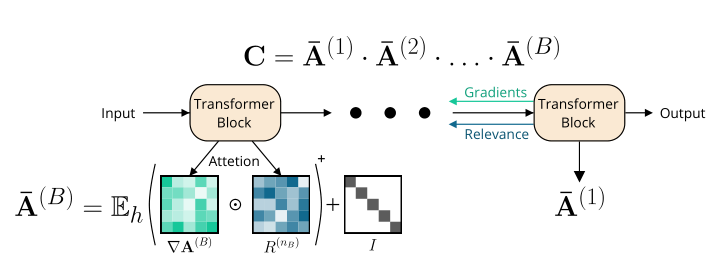
\includegraphics[width=15cm]{fig/ch2/trans1.png}
	\bicaption[\xiaosi Transformer attribution 计算过程]{\wuhao Transformer attribution 计算过程}{\wuhao Transformer attribution calculation procedure}
	\label{fig:trans1}
\end{figure}

\section{本章小结}
本章首先简要介绍了卷积神经网络和Transformer架构的基础原理,它们也是当前图像分类神经网络的两种主要基础架构。然后本章重点介绍了当前5种比较著名的显著图解释方法的背后原理和显著图生成的计算过程,这5种方法分别是Grad-CAM,Grad-CAM++,Score-CAM,LRP和Transformer a ttribution。这5种显著图解释方法也是第3章和第4章实验对比的其中一些方法。




